\input{../preamble.tex}

\SetDate[29/05/2026]

\usepackage{minted}

\def\arraystretch{2}
\setlength\tabcolsep{18pt}

\begin{document}
\pagestyle{fancy}
\fancyhead[L]{Seconde 5}
\fancyhead[C]{\textbf{Méthode de dichotomie}}
\fancyhead[R]{\today}

\section*{Le Juste Prix}

\subsection*{Règles du jeu}
%\begin{namedtheorem}[Règles du jeu]
	Le joueur doit deviner le prix d'un objet pour le gagner.
	Pour cela, il peut faire plusieurs estimations.
	%
	Le présentateur connaît le prix de l'objet. 
	À chaque estimation, il répond « C'est plus ! » ou \mbox{« C'est moins ! »} selon que le prix de l'objet est plus grand ou plus petit que l'estimation donnée.
	
	Le joueur est chronométré et doit trouver le prix exact de l'objet le plus vite possible.
%\end{namedtheorem}

% intéressant à comparer à l'oral ; pas la place pour l'écrit ici
%\subsection*{Méthode de balayage}

\subsection*{Méthode de dichotomie}

%\begin{namedtheorem}[Simplification]
	Supposons que le prix est un nombre entier entre 0€ et 1 000€ inclus.
%\end{namedtheorem}

\vspace{10pt}

\hspace{-40pt}
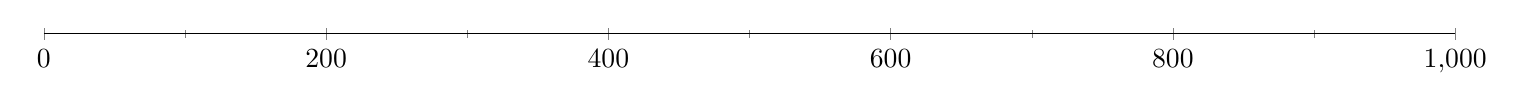
\begin{tikzpicture}
\begin{axis}[
	axis y line=none, 
	axis x line=middle, 
	axis line style=-,
	xmin=0, xmax=1000, 
	ymin=0, ymax=1,
	y=1pt,
	x=.51pt,
	xtick distance = 200,
	minor x tick num = 1,
	]
\end{axis}
\end{tikzpicture}


\hspace{-65pt}
\begin{tabular}{|*{12}{c|}}\hline
	Essai n° & 1 & 2 & 3 & 4 & 5 & 6 & 7 & 8 & 9 & 10 & 11
	\\\hline
	Estimation & & & & & & & & & & & 
	\\\hline
	Comparaison & & & & & & & & & & &
	\\\hline
\end{tabular}

\vspace{10pt}
Prix final trouvé :
\hspace{6cm}
Nombre d'estimations :

\vspace{10pt}

\hspace{-40pt}
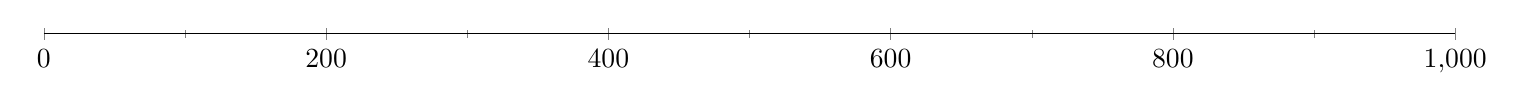
\begin{tikzpicture}
\begin{axis}[
	axis y line=none, 
	axis x line=middle, 
	axis line style=-,
	xmin=0, xmax=1000, 
	ymin=0, ymax=1,
	y=1pt,
	x=.51pt,
	xtick distance = 200,
	minor x tick num = 1,
	]
\end{axis}
\end{tikzpicture}

\hspace{-65pt}
\begin{tabular}{|*{12}{c|}}\hline
	Essai n° & 1 & 2 & 3 & 4 & 5 & 6 & 7 & 8 & 9 & 10 & 11
	\\\hline
	Estimation & & & & & & & & & & &
	\\\hline
	Comparaison & & & & & & & & & & &
	\\\hline
\end{tabular}

\vspace{10pt}
Prix final trouvé :
\hspace{6cm}
Nombre d'estimations :

\subsection*{Stratégie de dichotomie}
%\begin{namedtheorem}[Stratégie de dichotomie]
	
	\phantom{
	À chaque étape, on divise l'intervalle en deux et on appelle l'oracle pour exclure la moitié des valeurs candidates.
	}
	
	\phantom{
	Le nombre d'essais ne dépassera jamais 10 car $2^{10} = 1024 > 1000$.
	}
	
	%La stratégie est optimale car si l'oracle agit comme adversaire, il peut choisir de changer $P$ selon le prix $x$ proposé par le joueur.
%\end{namedtheorem}


\subsection*{Algorithme}
%\begin{namedtheorem}[Algorithme]\ \\
	\phantom{
	Entrée : fonction $f$ ; premier encadrement $a \leq x_0 \leq b$ ; précision $p$
	\\
	Sortie : encadrement final de $x_0$ tel que $b-a \leq p$
	\\
	Tant que $b-a > p$ : \\
		Calcul du milieu $m = \frac{a+b}2$ \\
		Appel à l'oracle pour connaitre le signe de $f(m)$ \\
		Si $f(m) > 0$ \\
		$b = m$ \\
		Sinon, \\
		$a = m$ 
	}
%\end{namedtheorem}

\newpage

\section*{Généralisation}

\subsection*{Problème de recherche de zéro}
%\begin{namedtheorem}[Problème de recherche de zéro]
	Toutes les équations peuvent se réécrire comme $f(x) = 0$.
	On appelle « \emph{zéro} de $f$ » ou « \emph{racine} de l'équation $f(x) = 0$ » un antécédent $x_0$ qui vérifie $f(x_0) = 0$.

	\begin{namedtheorem}[Problème]
	Étant donné une précision, comment obtenir un encadrement
		\mbox{$ a \leq x_0 \leq b $}
	d'amplitude $b-a$ inférieure à cette précision ?
	\end{namedtheorem}
%\end{namedtheorem}

\begin{multicols}{2}
	\begin{tikzpicture}[>=stealth, scale=1]
	\begin{axis}[xmin = 0, xmax=3, ymin=-8, ymax=2, axis x line=middle, axis y line=middle, axis line style = -, ytick distance=2, xtick distance=1, minor tick num=1, extra y ticks={0}, y=10pt, clip=false, ]
		\addplot[transparent, very thick, domain =0:3, samples=100] {x^2 - 7}  node[pos=.5, right] {$y=x^2 - 7$};
	\end{axis}
	\end{tikzpicture}
	\columnbreak
	\begin{namedtheorem}[Hypothèses]\
		\begin{itemize}[itemsep=5pt]
			\item
			Le tracé de $\C_f$ est continu : on trace la courbe sans lever son stylo.
			\item
			$f$ est croissante autour de son zéro : elle passe du négatif au positif autour $x_0$.
			% (on peut prendre $-f$ dans le cas contraire).
			\item
			%Pour chaque $x$ du domaine, un appel à un oracle permet de connaître le signe de $f(x)$.
			Il est facile de calculer le signe de $f(x)$.
		\end{itemize}
		\vfill\,
	\end{namedtheorem}
\end{multicols}


%Différence avec le balayage.

%\subsubsection*{Exemple 1}
%\python{while}
% Commentaires :
% 1. On initialise x = 0
% 2. Tant que x est strictement inférieur à 2
% 3. Remplacer x par sa valeur + 0,1
% 4. À la fin de la boucle, imprimer la valeur de x
% valeur attendue : 2
%
%Impression finale :
%
%Nombre d'itérations de la boucle \texttt{while} :
%
%\subsubsection*{Exemple 2}
%\python{while2}
% Commentaires :
% 1. On initialise x = 0
% 2. Tant que x est positif ou nul à 2
% 3. Remplacer x par sa valeur + 0,1
% 4. À la fin de la boucle, imprimer la valeur de x
% valeur attendue : boucle infinie !
%
%Impression finale :
%
%Nombre d'itérations de la boucle \texttt{while} :
%
%\newpage
%
%\exe{,difficulty=1}{
%	Compléter et implémenter le programme de balayage ci-dessous.
%	Que renvoie-t-il ?
%}{exe:balayage4}{
%	%\python{balayage-solution}
%}
%
%\python{balayage}
%
%
%\exe{}{
%	Donner la valeur de $\sqrt7$ à $10^{-5}$ près à l'aide d'un programme de balayage.
%}{exe:precision}{
%	En remplaçant la variable \texttt{amplitude} par \texttt{0.00001} ou \texttt{1e-5}, on obtient
%		\[ 2,64575 < \sqrt7 < 2,64576. \]
%	%\python{balayage-solution2}
%}
%
%\exe{}{
%	Donner la valeur de $\sqrt{700}$ à $10^{-4}$ près
%		\begin{enumerate}[label=\roman*)]
%			\item
%			à l'aide d'un programme de balayage ; et
%			\item
%			en montrant que $\sqrt{700} = 10\sqrt7$ et en utilisant l'exercice \ref{exe:precision}.
%		\end{enumerate}
%}{exe:precision2}{
%	En remplaçant la fonction $f$ par $f(x) = x^2 - 700$, et l'amplitude par $10^{-4}$, on obtient
%		\[ 26,4575 < \sqrt{700} < 26,4576. \]
%	%\python{balayage-solution3}
%	Comme $\sqrt{700} = \sqrt{100\times7} = \sqrt{100}\times\sqrt{7}=10\sqrt7$, on peut multiplier l'encadrement de l'exercice \ref{exe:precision} par 10 pour conclure immédiatement.
%}

\vspace{-40pt}

\subsection*{Trouver un polynôme annulateur}

\begin{namedtheorem}[Exemples]
	Considérons la fonction $f(x) = x^2 - 7$ (tracée ci-dessus). Elle est
	\begin{enumerate}
		\item un \emph{polynôme}, car elle s'exprime comme somme de multiples de $1, x, x^2, x^3, \hdots$ ; 
		\item \emph{annulatrice} de $\sqrt7$ car $f\bigl(\sqrt7\bigr) = 0$ ;
		\item à \emph{coefficients entiers} car les multiples de $1, x, x^2$ sont $-7 ; 0 ; 1$ respectivement et sont entiers.
	\end{enumerate}
	La fonction $g(x) = x-\sqrt7$ est un polynôme annulateur de $\sqrt7$ mais pas à coefficients entiers.
\end{namedtheorem}
	
\exe{, difficulty=0}{
	Trouver un polynôme à coefficients entiers et annulateur de $\sqrt2$.
}{exe:p-annul-sqrt2}{
	$f(x) = x^2 -2$ fonctionne, mais pas $f(x) = x-\sqrt2$ !
}
	
\exe{, difficulty=1}{
	Trouver un polynôme à coefficients entiers et annulateur de $\cos(30^\circ) = \frac{\sqrt3}2$.
}{exe:p-annul-sqrt32}{
	$g(x) = 4x^2 -3$ fonctionne, car $\frac{\sqrt3}2 = \sqrt{\frac34}$.
}
	
\exe{, difficulty=2}{
	Trouver un polynôme à coefficients entiers et annulateur à la fois de $\sqrt2$ et de $\frac{\sqrt3}2$.
}{exe:p-annul-sqrt2-sqrt32}{
	$h(x) = f(x)\cdot g(x) = (x^2 - 2)(4x^2 -3) = 4x^4 - 11x^2 + 6$ fonctionne, avec $f$ et $g$ des deux exercices précédents.
}


\exe{, difficulty=3}{
	Trouver un polynôme à coefficients entiers et annulateur de
		$ \sin(36\degree) = \sqrt{\frac{5-\sqrt5}8}. $

}{exe:p-annul}{
	En nommant $x = \sqrt{\dfrac{5-\sqrt5}8}$, la mise au carré donne
		\[ x^2 =  \dfrac{5-\sqrt5}8. \]
	En multipliant par 8 et en soustrayant 5, on trouve
		\begin{align*}
			 8x^2 &= 5 - \sqrt5, \\
			 8x^2 - 5 &= - \sqrt5.
		\end{align*}
	Une nouvelle mise au carré nous permet d'obtenir les égalités suivantes.
		\begin{align*}
			(8x^2 - 5)^2 &= 5 \\
			64x^4 - 80x^2 + 25 &= 5 \\
			64x^4 - 80x^2 + 20 &= 0 \\
			16x^4 - 20x^2 + 5 &= 0
		\end{align*}
	Un polynôme annulateur est donc $p(x) = 16x^4 - 20x^2 + 5$.
}

\begin{namedtheorem}[Théorème (très difficile)]
	Le nombre $\pi$, périmètre d'un cercle de diamètre 1, est un nombre transcendant : il n'existe pas de polynôme à coefficients entiers annulateur de $\pi$.
\end{namedtheorem}

\exe{, difficulty=4}{
	En supposant que $\pi$ est transcendant, montrer que $2\pi$ l'est aussi.
}{exe:2pi-transc}{
	Supposons, par contradiction, qu'il existe un polynôme à coefficients entiers annulant $2\pi$.
	Notons-le $a_0 + a_1x + \hdots + a_nx^n$ où les $a_0, a_1, \hdots, a_n \in\Z$ sont des entiers relatifs.
	
	Par hypothèse, $a_0 + a_1(2\pi) + a_2(2\pi)^2 + \hdots + a_n(2\pi)^n = 0$.
	Or, cette équation est équivalent à 
		\[ a_0 + (2a_1)\pi + (4a_2)\pi^2 + \hdots + (2^n a_n)\pi^n = 0, \]
	ce qui implique que $\pi$ est annulé par le polynôme $a_0 + 2a_1x + 4a_2x^2 + \hdots + 2^n a_n x^n$ dont les coefficients sont entiers relatifs car les $a_i$ sont des entiers relatifs.
	
	Nous obtenons une contradiction car $\pi$ est supposé transcendant : $2\pi$ l'est donc également.
}

\subsection*{Étude de complexité}


\exe{, difficulty=2}{
	En partant d'un encadrement à l'unité d'un zéro, combien d'étapes faut-il pour calculer ses 10 premières décimales ?
	
	Montrer qu'on cherche le plus petit $n\in\N$ tel que $2^{n} > 10^{10}$
	puis concevoir un algorithme permettant de trouver $n$.
	L'implémenter et vérifier qu'on obtient bien $n=34$.
}{exe:appf4}{
	Algorithme Python naïf : tant que $2^n < 10^{10}$, ajouter 1 à $n$.
	
	Cependant cet algorithme nécessite de calculer $10^{10}$ et donc de le représenter en base 2. Or, la longueur de cette représentation est exactement $n$.
	
	Algorithme sur machine de Turing : écrire $10$ en base 2, calculer $10^{10}$ avec 4 multiplications
		\[ 10^{10} = \left(\left((10)^2\right)^2\right)^2 \times 10^2 \]
	puis regarder la longueur de la représentation binaire.
	
}

\exe{, difficulty=2}{
	Montrer que l'algorithme par dichotomie sur la fonction $f(x) = x^2 - 2$ avec encadrement de départ $1 \leq x_0 \leq 2$ et précision $p=0$ ne termine jamais.
	
	\emph{Indication : montrer que les bornes calculées sont toujours rationnelles alors que $\sqrt2$ ne l'est pas.}
}{exe:appf1}{
	L'encadrement $[1;2]$ de départ est rationnel.
	De plus, à chaque étape, si l'encadrement est rationnel, le prochain le sera aussi.
	En effet, le milieu de $\left[\frac{a}b ; \frac{p}q\right]$ est
		\[ m = \frac12 \left(\frac{a}b + \frac{p}q\right) = \frac{aq + bp}{2bq} \in \Q, \]
	qui est toujours rationnel.
	
	La racine de $f$ située dans $[1;2]$ est bien sûr $\sqrt2$.
	Dès lors, un encadrement $a \leq \sqrt2 \leq b$ d'amplitude $b-a=0$ correspond à obtenir $a=b=\sqrt2$, car $b-a = 0 \iff a = b$.
	
	Or, $\sqrt2$ est irrationnel d'après le cours, et donc l'algorithme ne peut pas aboutir.
}


%%%%%%%%%%%

\newpage
\fancyhead[C]{\textbf{Solutions}}
\shipoutAnswer

\end{document}
